\documentclass[10pt,landscape]{article}
\usepackage{multicol}
\usepackage{calc}
\usepackage{ifthen}
\usepackage[landscape]{geometry}
\usepackage{amsmath,amsthm,amsfonts,amssymb}
\usepackage{color,graphicx,overpic}
\usepackage{hyperref}
\usepackage{graphicx}
\usepackage{amsmath}
\graphicspath{ {sheet_images/} }

%Originally Modified by Daniel Kenner for Calc 3 Cheat Sheet
%Template Originally found @ http://tex.stackexchange.com/questions/8827/preparing-cheat-sheets
%Conic images originally found on google images when looking for named shapes

\pdfinfo{
  /Title (Calculus 3 Cheat Sheet.pdf)
  /Creator (TeX)
  /Producer (pdfTeX 1.40.0)
  /Author (Daniel Kenner)
  /Subject (Example)
  /Keywords (pdflatex, latex,pdftex,tex)}

% This sets page margins to .5 inch if using letter paper, and to 1cm
% if using A4 paper. (This probably isn't strictly necessary.)
% If using another size paper, use default 1cm margins.
\ifthenelse{\lengthtest { \paperwidth = 11in}}
    { \geometry{top=.25in,left=.25in,right=.25in,bottom=.25in} }
    {\ifthenelse{ \lengthtest{ \paperwidth = 297mm}}
        {\geometry{top=1cm,left=1cm,right=1cm,bottom=1cm} }
        {\geometry{top=1cm,left=1cm,right=1cm,bottom=1cm} }
    }

% Turn off header and footer
\pagestyle{empty}

% Redefine section commands to use less space
\makeatletter
\renewcommand{\section}{\@startsection{section}{1}{0mm}%
                                {-1ex plus -.5ex minus -.2ex}%
                                {0.5ex plus .2ex}%x
                                {\normalfont\large\bfseries}}
\renewcommand{\subsection}{\@startsection{subsection}{2}{0mm}%
                                {-1explus -.5ex minus -.2ex}%
                                {0.5ex plus .2ex}%
                                {\normalfont\normalsize\bfseries}}
\renewcommand{\subsubsection}{\@startsection{subsubsection}{3}{0mm}%
                                {-1ex plus -.5ex minus -.2ex}%
                                {1ex plus .2ex}%
                                {\normalfont\small\bfseries}}
\makeatother

% Define BibTeX command
\def\BibTeX{{\rm B\kern-.05em{\sc i\kern-.025em b}\kern-.08em
    T\kern-.1667em\lower.7ex\hbox{E}\kern-.125emX}}

% Don't print section numbers
\setcounter{secnumdepth}{0}


\setlength{\parindent}{0pt}
\setlength{\parskip}{0pt plus 0.5ex}

%My Environments
\newtheorem{example}[section]{Example}
% -----------------------------------------------------------------------

\begin{document}
\raggedright
\footnotesize
\begin{multicols*}{5}


% multicol parameters
% These lengths are set only within the two main columns
%\setlength{\columnseprule}{0.25pt}
\setlength{\premulticols}{1pt}
\setlength{\postmulticols}{1pt}
\setlength{\multicolsep}{1pt}
\setlength{\columnsep}{2pt}

\section{Derivatives}
\scriptsize
$D_x e^x=e^x$\newline
$D_x \sin(x)=\cos(x)$\newline
$D_x \cos(x)=-\sin(x)$\newline
$D_x \tan(x)=\sec^2(x)$\newline
$D_x \cot(x)=-\csc^2(x)$\newline
$D_x \sec(x)=\sec(x)\tan(x)$\newline
$D_x \csc(x)=-\csc(x)\cot(x)$\newline
$D_x \sin^{-1}=\frac{1}{\sqrt{1-x^2}}, x \in [-1,1]$\newline
$D_x \cos^{-1}=\frac{-1}{\sqrt{1-x^2}}, x \in [-1,1]$\newline
$D_x \tan^{-1}=\frac{1}{1+x^2}, \frac{-\pi}{2}\le x \le \frac{\pi}{2}$\newline
$D_x \sec^{-1}=\frac{1}{\mid x \mid \sqrt{x^2-1}}, |x| > 1$\newline
$D_x \sinh(x)=\cosh(x)$\newline
$D_x \cosh(x)=\sinh(x)$\newline
$D_x \tanh(x)=sech^2(x)$\newline
$D_x \coth(x)=-csch^2(x)$\newline
$D_x sech(x)=-sech(x)\tanh(x)$\newline
$D_x csch(x)=-csch(x)\coth(x)$\newline
$D_x \sinh^{-1}=\frac{1}{\sqrt{x^2+1}}$\newline
$D_x \cosh^{-1}=\frac{-1}{\sqrt{x^2-1}}, x > 1$\newline
$D_x \tanh^{-1}=\frac{1}{1-x^2} -1 < x < 1$\newline
$D_x sech^{-1}=\frac{1}{x \sqrt{1-x^2}}, 0 < x < 1$
$ D_x \ln(x) = \frac{1}{x} $

\section{Integrals}
\scriptsize
$\int \frac{1}{x}dx = \ln|x|+c$\newline
$\int e^x dx = e^x+c $\newline
$\int a^x dx = \frac{1}{\ln a} a^x+c $\newline
$\int e^{ax} dx = \frac{1}{a} e^{ax}+c $\newline
$\int \frac{1}{\sqrt{1-x^2}} dx = \sin^{-1}(x)+c $\newline
$\int \frac{1}{1+x^2} dx = \tan^{-1}(x)+c $\newline
$\int \frac{1}{x\sqrt{x^2-1}} dx = \sec^{-1}(x)+c $\newline
$\int \sinh(x) dx = \cosh(x)+c $\newline
$\int \cosh(x) dx = \sinh(x)+c $\newline
$\int \tanh(x) dx = \ln|\cosh(x)|+c $\newline
$\int \tanh(x)sech(x) dx = -sech(x)+c $\newline
$\int sech^2(x) dx = \tanh(x)+c $\newline
$\int csch(x)\coth(x) dx = -csch(x)+c $\newline
$\int \tan(x) dx = -\ln|\cos(x) |+c $\newline
$\int \cot(x) dx = \ln|\sin(x)|+c $\newline
$\int \cos(x) dx = \sin(x)+c $\newline
$\int \sin(x) dx = -\cos(x)+c $\newline
$\int \frac{1}{\sqrt{a^2-u^2}} dx = \sin^{-1}(\frac{u}{a})+c $\newline
$\int \frac{1}{a^2+u^2} dx = \frac{1}{a}\tan^{-1}\frac{u}{a}+c $\newline
$ \int ln(x) dx = (xln(x))-x+c $\newline

\textbf{U-Substitution}\newline
Let $ u=f(x) $ (can be more than one variable).\newline
Determine: $ du = \frac{f(x)}{dx}dx $ and solve for dx.\newline
Then, if a definite integral, substitute the bounds for $ u=f(x) $ at each bounds\newline
Solve the integral using u.\newline

\textbf{Integration by Parts}\newline
$ \int u dv = uv-\int v du $

\section{Fns and Identities}
$\sin(\cos^{-1}(x)) = \sqrt{1-x^2}$\newline
$\cos(\sin^{-1}(x)) = \sqrt{1-x^2} $\newline
$\sec(\tan^{-1}(x)) = \sqrt{1+x^2} $\newline
$\tan(\sec^{-1}(x)) \newline = (\sqrt{x^2-1} \: $if$ \: x \ge 1)\newline =(-\sqrt{x^2-1} \: if \: x \le -1)$
$\sinh^{-1}(x) = \ln{x+\sqrt{x^2+1}} $\newline
$\sinh^{-1}(x) = \ln{x+\sqrt{x^2-1}}, \: x \ge -1 $\newline
$\tanh^{-1}(x) = \frac{1}{2}\ln{x+\frac{1+x}{1-x}}, \: 1 < x < -1 $\newline
$sech^{-1}(x) = \ln[{\frac{1+\sqrt{1-x^2}}{x}}], \: 0 < x \le -1 $\newline
$\sinh(x) = \frac{e^{x}-e^{-x}}{2} $\newline
$\cosh(x) = \frac{e^{x}+e^{-x}}{2} $

\section{Trig Identities}
$ \sin^2(x)+\cos^2(x) = 1 $\newline
$ 1+\tan^2(x) = \sec^2(x) $\newline
$ 1+\cot^2(x) = \csc^2(x) $\newline
$ \sin(x\pm y) = \sin(x)\cos(y)\pm\cos(x)\sin(y) $\newline
$ \cos(x\pm y) = \cos(x)\cos(y)\pm\sin(x)\sin(y) $\newline
$ \tan(x\pm y) = \frac{\tan(x)\pm\tan(y)}{1 \mp \tan(x)\tan(y)} $\newline
$ \sin(2x) = 2\sin(x)\cos(x) $\newline
$ \cos(2x) = \cos^{2}(x) - \sin^{2}(x) $\newline
$ \cosh(n^{2}x)-\sinh^{2}x = 1 $\newline
$ 1+\tan^2(x) = \sec^2(x) $\newline
$ 1+\cot^2(x) = \csc^2(x) $\newline
$ \sin^2(x) = \frac{1-\cos(2x)}{2} $\newline
$ \cos^2(x) = \frac{1+\cos(2x)}{2} $\newline
$ \tan^2(x) = \frac{1-\cos(2x)}{1+\cos(2x)} $\newline
$ \sin(-x) = -\sin(x) $\newline
$ \cos(-x) = \cos(x) $\newline
$ \tan(-x) = -\tan(x) $

\section {Calculus 3 Concepts}

\subsection{Cartesian coords in 3D}
given two points:\newline
$ (x_1, y_1, z_1) $ and $ (x_2, y_2, z_2)$,\newline
Distance between them:\newline
$ \sqrt{(x_1-x_2)^2+(y_1-y_2)^2+(z_1-z_2)^2} $\newline
Midpoint:\newline
$ (\frac{x_1+x_2}{2},\frac{y_1+y_2}{2},\frac{z_1+z_2}{2}) $\newline
Sphere with center (h,k,l) and radius r:\newline
$ (x-h)^2 + (y-k)^2 + (z-l)^2 = r^2 $

\subsection{Vectors}
Vector: $ \vec{u} $\newline
Unit Vector: $ \hat{u} $\newline
Magnitude: $ ||\vec{u}|| = \sqrt{u_1^2+u_2^2+u_3^2}$\newline
Unit Vector: $ \hat{u} = \frac{\vec{u}}{||\vec{u}||} $\newline

\textbf{Dot Product}\newline
$ \vec{u} \cdot \vec{v} $\newline
Produces a Scalar \newline
(Geometrically, the dot product is a vector projection)\newline
$\vec{u} = < u_1, u_2, u_3 >$\newline
$\vec{v} = < v_1, v_2, v_3 >$\newline
$ \vec{u} \cdot \vec{v} = \vec{0} $ means the two vectors are Perpendicular
$ \theta $ is the angle between them.\newline
$\vec{u} \cdot \vec{v} = ||\vec{u}||\:||\vec{v}||\cos(\theta) $\newline
$\vec{u} \cdot \vec{v} = u_1v_1 + u_2v_2 + u_3v_3 $\newline
NOTE:\newline
$ \hat{u} \cdot \hat{v} = \cos(\theta) $\newline
$ ||\vec{u}||^2 = \vec{u} \cdot \vec{u} $\newline
$ \vec{u} \cdot \vec{v} = 0 $ when $ \bot $\newline
Angle Between $ \vec{u} $ and $ \vec{v} $:\newline
$ \theta = \cos^{-1}(\frac{\vec{u} \cdot \vec{v}}{||\vec{u}||\:||\vec{v}||}) $\newline
Projection of $ \vec{u} $ onto $ \vec{v} $:\newline
$ pr_{\vec{v}}\vec{u} = (\frac{\vec{u} \cdot \vec{v}}{||\vec{v}||^2})\vec{v} $\newline

\textbf{Cross Product}\newline
$\vec{u} \times \vec{v}$\newline
Produces a Vector\newline
(Geometrically, the cross product is the area of a paralellogram with sides $ ||\vec{u}|| $ and $ ||\vec{v}|| $)\newline
$\vec{u} = < u_1, u_2, u_3 >$\newline
$\vec{v} = < v_1, v_2, v_3 >$\newline
\[
\vec{u} \times \vec{v} = 
\begin{vmatrix}
\hat{i} & \hat{j} & \hat{k} \\
u_1 & u_2 & u_3 \\
v_1 & v_2 & v_3
\end{vmatrix}
\]\newline 
$ \vec{u} \times \vec{v} = \vec{0} $ means the vectors are paralell

\subsection {Lines and Planes}
\textbf{Equation of a Plane}\newline
$ (x_0, y_0, z_0) $ is a point on the plane and $ <A,B,C> $ is a normal vector\newline

$A(x-x_0)+B(y-y_0)+C(z-z_0) = 0$\newline
$ <A,B,C> \cdot <x-x_0, y-y_0, z-z_0> = 0 $\newline
$ Ax+By+Cz = D $ where $ D=Ax_0+By_0+Cz_0 $\newline

\textbf{Equation of a line}\newline
A line requires a Direction Vector $ \vec{u}=<u_1,u_2,u_3> $ and a point $(x_1,y_1,z_1)$\newline
then,\newline a parameterization of a line could be:\newline
$ x = u_1t+x_1 $\newline
$ y = u_2t+y_1 $\newline
$ z = u_3t+z_1 $\newline

\textbf{Distance from a Point to a Plane}\newline
The distance from a point $(x_0,y_0,z_0)$ to a plane Ax+By+Cz=D can be expressed by the formula:\newline
$ d=\frac{|Ax_0+By_0+Cz_0-D|}{\sqrt{A^2+B^2+C^2}} $\newline


\subsection { Coord Sys Conv }
\textbf{Cylindrical to Rectangular}\newline
$ x=r\cos(\theta) $\newline
$ y=r\sin(\theta) $\newline
$ z=z $\newline
\textbf{Rectangular to Cylindrical}\newline
$ r=\sqrt{x^2+y^2} $\newline
$ \tan(\theta) = \frac{y}{x} $\newline
$ z=z $\newline
\textbf{Spherical to Rectangular}\newline
$ x=\rho\sin(\phi)\cos(\theta) $\newline
$ y=\rho\sin(\phi)\sin(\theta) $\newline
$ z=\rho\cos(\phi) $\newline
\textbf{Rectangular to Spherical}\newline
$ \rho=\sqrt{x^2+y^2+z^2} $\newline
$ \tan(\theta) = \frac{y}{x} $\newline
$ \cos(\phi) = \frac{z}{\sqrt{x^2+y^2+z^2}} $\newline
\textbf{Spherical to Cylindrical}\newline
$ r=\rho\sin(\phi) $\newline
$ \theta=\theta $\newline
$ z=\rho\cos(\phi) $\newline
\textbf{Cylindrical to Spherical}\newline
$ \rho=\sqrt{r^2+z^2} $\newline
$ \theta=\theta $\newline
$ \cos(\phi) = \frac{z}{\sqrt{r^2+z^2}} $

\subsection{Surfaces}
\textbf{Ellipsoid}\newline
$ \frac{x^2}{a^2}+\frac{y^2}{b^2}+\frac{z^2}{c^2} = 1 $\newline
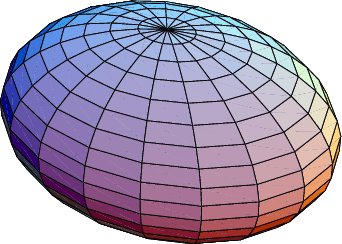
\includegraphics[scale=0.15]{ellipsoid}\newline
\textbf{Hyperboloid of One Sheet}\newline
$ \frac{x^2}{a^2}+\frac{y^2}{b^2}-\frac{z^2}{c^2} = 1 $\newline
(Major Axis: z because it follows - )\newline
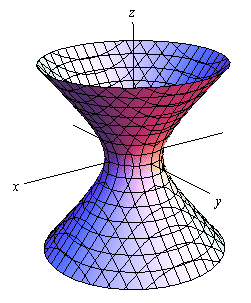
\includegraphics[scale=0.15]{hyperboloid1}\newline
\textbf{Hyperboloid of Two Sheets}\newline
$ \frac{z^2}{c^2}-\frac{x^2}{a^2}-\frac{y^2}{b^2} = 1 $\newline
(Major Axis: Z because it is the one not subtracted)\newline
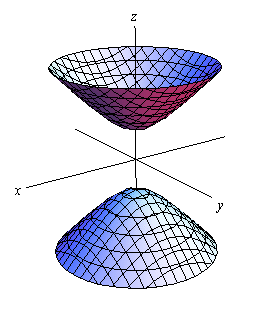
\includegraphics[scale=0.15]{hyperboloid2}\newline
\textbf{Elliptic Paraboloid}\newline
$ z=\frac{x^2}{a^2}+\frac{y^2}{b^2} $\newline
(Major Axis: z because it is the variable NOT squared)\newline
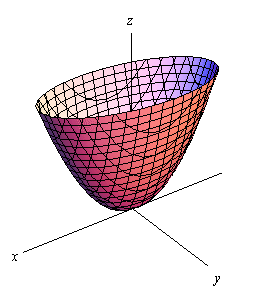
\includegraphics[scale=0.15]{elliptic_paraboloid}\newline
\textbf{Hyperbolic Paraboloid}\newline
(Major Axis: Z axis because it is not squared)\newline
$ z=\frac{y^2}{b^2}-\frac{x^2}{a^2} $\newline
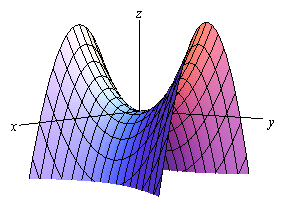
\includegraphics[scale=0.15]{hyperbolic_paraboloid}\newline
\textbf{Elliptic Cone}\newline
(Major Axis: Z axis because it's the only one being subtracted)\newline
$ \frac{x^2}{a^2}+\frac{y^2}{b^2}-\frac{z^2}{c^2} = 0 $\newline
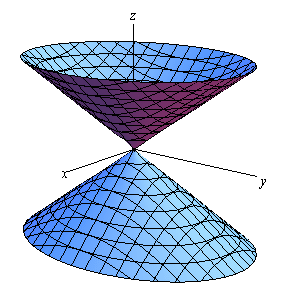
\includegraphics[scale=0.15]{elliptic_cone}\newline
\textbf{Cylinder}\newline
1 of the variables is missing\newline
OR\newline
$ (x-a)^2+(y-b^2) = c $\newline
(Major Axis is missing variable)

\subsection{Partial Derivatives}
Partial Derivatives are simply holding all other variables constant (and act like constants for the derivative) and only taking the derivative with respect to a given variable.\newline
Given z=f(x,y), the partial derivative of z with respect to x is:\newline
$f_x(x,y) = z_x = \frac{\partial z}{\partial x} = \frac{\partial f(x,y)}{\partial x}$\newline
likewise for partial with respect to y:\newline
$f_y(x,y) = z_y = \frac{\partial z}{\partial y} = \frac{\partial f(x,y)}{\partial y}$\newline
\textbf{Notation}\newline
For $ f_{xyy} $, work "inside to outside" $ f_{x} $ then $ f_{xy} $, then $ f_{xyy} $\newline
$f_{xyy} = \frac{\partial^3 f}{\partial x \partial^2 y}, $\newline
For $\frac{\partial^3 f}{\partial x \partial^2 y}$ , work right to left in the denominator

\subsection {Gradients}
The Gradient of a function in 2 variables is $ \nabla f = < f_x, f_y > $\newline
The Gradient of a function in 3 variables is $ \nabla f = < f_x, f_y, f_z > $

\subsection {Chain Rule(s)}

Take the Partial derivative with respect to the first-order variables of the function times the partial (or normal) derivative of the first-order variable to the ultimate variable you are looking for summed with the same process for other first-order variables this makes sense for.\newline
Example:\newline
let x = x(s,t), y = y(t) and z = z(x,y).\newline
z then has first partial derivative:\newline
$ \frac{\partial z}{\partial x} $ and $ \frac{\partial z}{\partial y} $ \newline
x has the partial derivatives:\newline
$ \frac{\partial x}{\partial s} $ and $ \frac{\partial x}{\partial t} $ \newline
and y has the derivative:\newline
$ \frac{dy}{dt} $ \newline
In this case (with z containing x and y as well as x and y both containing s and t), the chain rule for $ \frac{\partial z}{\partial s} $ is $ \frac{\partial z}{\partial s} = \frac{\partial z}{\partial x} \frac{\partial x}{\partial s} $\newline
The chain rule for $ \frac{\partial z}{\partial t} $ is $ \frac{\partial z}{\partial t} = \frac{\partial z}{\partial x} \frac{\partial x}{\partial t} + \frac{\partial z}{\partial y} \frac{dy}{dt}$\newline
Note: the use of "d" instead of $ "\partial" $ with the function of only one independent variable

\subsection{Limits and Continuity}
\textbf{Limits in 2 or more variables}\newline
Limits taken over a vectorized limit just evaluate separately for each component of the limit.\newline
\textbf{Strategies to show limit exists}\newline
1. Plug in Numbers, Everything is Fine\newline
2. Algebraic Manipulation\newline
-factoring/dividing out\newline
-use trig identites\newline
3. Change to polar coords\newline
\:\:$if (x,y)\to(0,0)\Leftrightarrow r\to0$\newline
\textbf{Strategies to show limit DNE}\newline
1. Show limit is different if approached from different paths\newline
(x=y, $x=y^2,$ etc.)\newline
2. Switch to Polar coords and show the limit DNE.\newline
\textbf{Continunity}\newline
A fn, $z=f(x,y)$, is continuous at (a,b) if\newline
$f(a,b) = \lim_{(x,y) \to (a,b)} f(x,y) $\newline
Which means:\newline
1. The limit exists\newline
2. The fn value is defined\newline
3. They are the same value

\subsection{Directional Derivatives}
Let z=f(x,y) be a fuction, (a,b) ap point in the domain (a valid input point) and $ \hat{u} $ a unit vector (2D).\newline
The Directional Derivative is then the derivative at the point (a,b) in the direction of $ \hat{u} $ or:\newline
$ D_{\vec{u}}f(a,b) = \hat{u} \cdot \nabla f(a,b)$\newline
This will return a \textit{scalar}.
4-D version: $ D_{\vec{u}}f(a,b,c) = \hat{u} \cdot \nabla f(a,b,c) $

\subsection{Tangent Planes}
let F(x,y,z) = k be a surface and P = $(x_0, y_0, z_0)$ be a point on that surface.\newline
Equation of a Tangent Plane:\newline
$ \nabla F(x_0,y_0,z_0) \cdot <x-x_0, y-y_0, z-z_0> $

\subsection {Approximations}
let $ z=f(x,y) $ be a differentiable function
total differential of f = dz\newline
$dz= \nabla f \cdot < dx, dy >$\newline
This is the \textit{approximate} change in z\newline
The actual change in z is the difference in z values:\newline
$ \Delta z = z-z_1 $

\subsection {Maxima and Minima}
\textbf{Internal Points}\newline
1. Take the Partial Derivatives with respect to X and Y ($ f_x $ and $ f_y $) (Can use gradient)\newline
2. Set derivatives equal to 0 and use to solve system of equations for x and y\newline
3. Plug back into original equation for z.\newline
Use Second Derivative Test for whether points are local max, min, or saddle\newline

\textbf{Second Partial Derivative Test}\newline
1. Find all (x,y) points such that $ \nabla f(x,y) = \vec{0} $\newline
2. Let $ D=f_{xx}(x,y)f_{yy}(x,y)-f_{xy}^2(x,y) $\newline
IF (a) D $>$ 0 AND $ f_{xx} < 0, $ f(x,y) is local max value\newline
(b) D $>$ 0 AND $f_{xx}(x,y) > 0$ f(x,y) is local min value\newline
(c) D $<$ 0, (x,y,f(x,y)) is a saddle point\newline
(d) D $=$ 0, test is inconclusive\newline
3. Determine if any boundary point gives min or max. Typically, we have to parametrize boundary and then reduce to a Calc 1 type of min/max problem to solve.

\textbf{The following only apply only if a boundary is given}\newline
1. check the corner points\newline
2. Check each line (0 $\le$ x $\le$ 5 would give x=0 and x=5 )\newline
On Bounded Equations, this is the global min and max...second derivative test is not needed.

\subsection{Lagrange Multipliers}
Given a function f(x,y) with a constraint g(x,y), solve the following system of equations to find the max and min points on the constraint (NOTE: may need to also find internal points.):\newline
$ \nabla f = \lambda \nabla g $\newline
$ g(x,y) = 0 (or k if given) $

\subsection{Double Integrals}
With Respect to the xy-axis, if taking an integral,\newline
$ \int\int dy dx $ is cutting in vertical rectangles,\newline
$ \int\int dx dy $ is cutting in horizontal rectangles\newline

\textbf{Polar Coordinates}\newline
When using polar coordinates, $ dA = r dr  d\theta $

\subsection{Surface Area of a Curve}
let z = f(x,y) be continuous over S (a closed Region in 2D domain)\newline
Then the surface area of z = f(x,y) over S is:\newline
$ SA = \int\int_S\sqrt{f_x^2+f_y^2+1} dA $

\subsection {Triple Integrals}
$ \int\int\int_s f(x,y,z)dv = \int_{a_1}^{a_2}\int_{\phi_1(x)}^{\phi_2(x)}\int_{\psi_1(x,y)}^{\psi_2(x,y)} f(x,y,z)dzdydx $\newline
Note: $ dv $ can be exchanged for $ dxdydz $ in any order, but you must then choose your limits of integration according to that order

\subsection {Jacobian Method}
$ \int\int_Gf(g(u,v),h(u,v)) | J(u,v) | du dv = \int\int_R f(x,y) dx dy $\newline
\[
J(u,v) = 
\begin{vmatrix}
\frac{\partial x}{\partial u} & \frac{\partial x}{\partial v} \\
\frac{\partial y}{\partial u} & \frac{\partial y}{\partial v}
\end{vmatrix}
\]\newline
Common Jacobians:\newline
Rect. to Cylindrical: $r$\newline
Rect. to Spherical: $\rho^2 \sin(\phi)$

\subsection {Vector Fields}
%note, this one should be moved around so that it is on the last column...it's kinda big.
let $ f(x,y,z) $ be a scalar field and $ \vec{F}(x,y,z) = M(x,y,z)\hat{i} + N(x,y,z)\hat{j} + P(x,y,z)\hat{k} $ be a vector field,\newline
Grandient of f = $ \nabla f = < \frac{\partial f}{\partial x}, \frac{\partial f}{\partial y}, \frac{\partial f}{\partial z} >$\newline
Divergence of $ \vec{F}$:\newline $ \nabla\cdot\vec{F} = \frac{\partial M}{\partial x} + \frac{\partial N}{\partial y} + \frac{\partial P}{\partial z} $\newline
Curl of $ \vec{F}$:\newline $ \nabla\times\vec{F} = 
\begin{vmatrix}
\hat{i} & \hat{j} & \hat{k} & \\
\frac{\partial}{\partial x} & \frac{\partial}{\partial y} & \frac{\partial}{\partial z} \\
M & N & P
\end{vmatrix} $

\subsection{Line Integrals}
C given by $x = x(t), y = y(t), t\in [a,b]$\newline 
$ \int_cf(x,y)ds = \int_a^bf(x(t), y(t)) ds $\newline
where $ ds = \sqrt{(\frac{dx}{dt})^2+(\frac{dy}{dt})^2} dt $\newline
or $ \sqrt{1+(\frac{dy}{dx})^2} dx $\newline
or $ \sqrt{1+(\frac{dx}{dy})^2} dy $\newline
To evaluate a Line Integral,\newline
$\cdot$ get a paramaterized version of the line (usually in terms of t, though in exclusive terms of x or y is ok)\newline
$\cdot$ evaluate for the derivatives needed (usually dy, dx, and/or dt)\newline
$\cdot$ plug in to original equation to get in terms of the independant variable\newline
$\cdot$ solve integral\newline

\textbf{Work}\newline
Let $ \vec{F} = M\hat{i}+\hat{j}+\hat{k} $ (force) $ M=M(x,y,z), N=N(x,y,z), P=P(x,y,z) $\newline
(Literally)$ d\vec{r} = dx\hat{i}+dy\hat{j}+dz\hat{k} $\newline
Work $ w = \int_c\vec{F}\cdot d\vec{r} $\newline
(Work done by moving a particle over curve C with force $ \vec{F} $)

\subsection{Independence of Path}
\textbf{Fund Thm of Line Integrals}\newline
C is curve given by $ \vec{r}(t), t\in[a,b];\newline \vec{r}\prime(t) $ exists. If $ f(\vec{r}) $ is continuously differentiable on an open set containing C, then $ \int_c\nabla f(\vec{r}) \cdot d\vec{r} = f(\vec{b}) - f(\vec{a}) $\newline
\textbf{Equivalent Conditions}\newline
$ \vec{F}(\vec{r}) $ continuous on open connected set D. Then,\newline
$ (a) \vec{F} = \nabla f $ for some fn f. (if $ \vec{F} $ is conservative)
$ \Leftrightarrow (b) \int_c\vec{F}(\vec{r})\cdot d\vec{r} is indep. of path in D $\newline
$ \Leftrightarrow (c) \int_c\vec{F}(\vec{r})\cdot d\vec{r} = 0 $ for all closed paths in D.\newline
\textbf{Conservation Theorem}\newline
$ \vec{F} = M\hat{i}+N\hat{j}+P\hat{k} $ continuously differentiable on open, simply connected set D.\newline
$ \vec{F} $ conservative $ \Leftrightarrow \nabla\times\vec{F} = \vec{0} $ \newline
(in 2D $ \nabla\times\vec{F}=\vec{0} $ iff $ M_y = N_x$)

\subsection{Green's Theorem}
(method of changing line integral for double integral - Use for Flux and Circulation across 2D curve and line integrals over a closed boundary)\newline
$ \oint Mdy - Ndx = \int\int_R(M_x+N_y)dxdy $\newline
$ \oint Mdx + Ndy = \int\int_R (N_x-M_y) dxdy $\newline
Let:\newline
$\cdot$R be a region in xy-plane\newline
$\cdot$C is simple, closed curve enclosing R (w/ paramerization $ \vec{r}(t) $)\newline
$ \cdot\vec{F}(x,y) = M(x,y)\hat{i} + N(x,y)\hat{j} $ be continuously differentiable over R$\cup$C. \newline
\textbf{Form 1: Flux Across Boundary}\newline
$ \vec{n} = $ unit normal vector to C\newline
$ \oint_c \vec{F}\cdot\vec{n} = \int\int_R \nabla\cdot\vec{F} dA $\newline
$ \Leftrightarrow\oint Mdy - Ndx = \int\int_R(M_x+N_y)dxdy $\newline
\textbf{Form 2: Circulation Along Boundary}\newline
$ \oint_c\vec{F}\cdot d\vec{r} = \int\int_R \nabla\times\vec{F}\cdot\hat{u} dA $\newline
$ \Leftrightarrow \oint Mdx + Ndy = \int\int_R (N_x-M_y) dxdy $\newline
\textbf{Area of R}\newline
$ A = \oint(\frac{-1}{2}y dx + \frac{1}{2}x dy) $

\subsection{Gauss' Divergence Thm}
(3D Analog of Green's Theorem - Use for Flux over a 3D surface)
Let:\newline
$ \cdot\vec{F}(x,y,z) $ be vector field continuously differentiable in solid S\newline
$ \cdot $S is a 3D solid
$ \cdot\partial S $ boundary of S (A Surface)\newline
$ \cdot\hat{n} $unit outer normal to $ \partial S $\newline
Then,\newline
$ \int\int_{\partial S}\vec{F}(x,y,z)\cdot\hat{n}dS = \int\int\int_S\nabla\cdot\vec{F} dV $\newline
(dV = dxdydz)

\vfill\columnbreak

\subsection{Surface Integrals}
Let\newline
$\cdot$R be closed, bounded region in xy-plane\newline
$\cdot$f be a fn with first order partial derivatives on R\newline
$\cdot$G be a surface over R given by $ z=f(x,y) $\newline
$\cdot g(x,y,z) = g(x,y,f(x,y))$ is cont. on R\newline
Then,\newline$ \int\int_G g(x,y,z) dS = \int\int_R g(x,y,f(x,y)) dS $\newline
where $ dS = \sqrt{f_x^2+f_y^2+1}dydx $\newline
\textbf{Flux of $ \vec{F} $ across G}\newline
$ \int\int_G\vec{F}\cdot{n} dS = \int\int_R[-Mf_x-Nf_y+P]dxdy $\newline
where:\newline
$\cdot\vec{F}(x,y,z) = M(x,y,z)\hat{i} + N(x,y,z)\hat{j} + P(x,y,z)\hat{k} $\newline
$\cdot$G is surface f(x,y)=z\newline
$\cdot\vec{n}$ is upward unit normal on G.\newline
$\cdot$f(x,y) has continuous $1^{st}$ order partial derivatives
\vfill
\subsection{Unit Circle}
(cos, sin)\newline
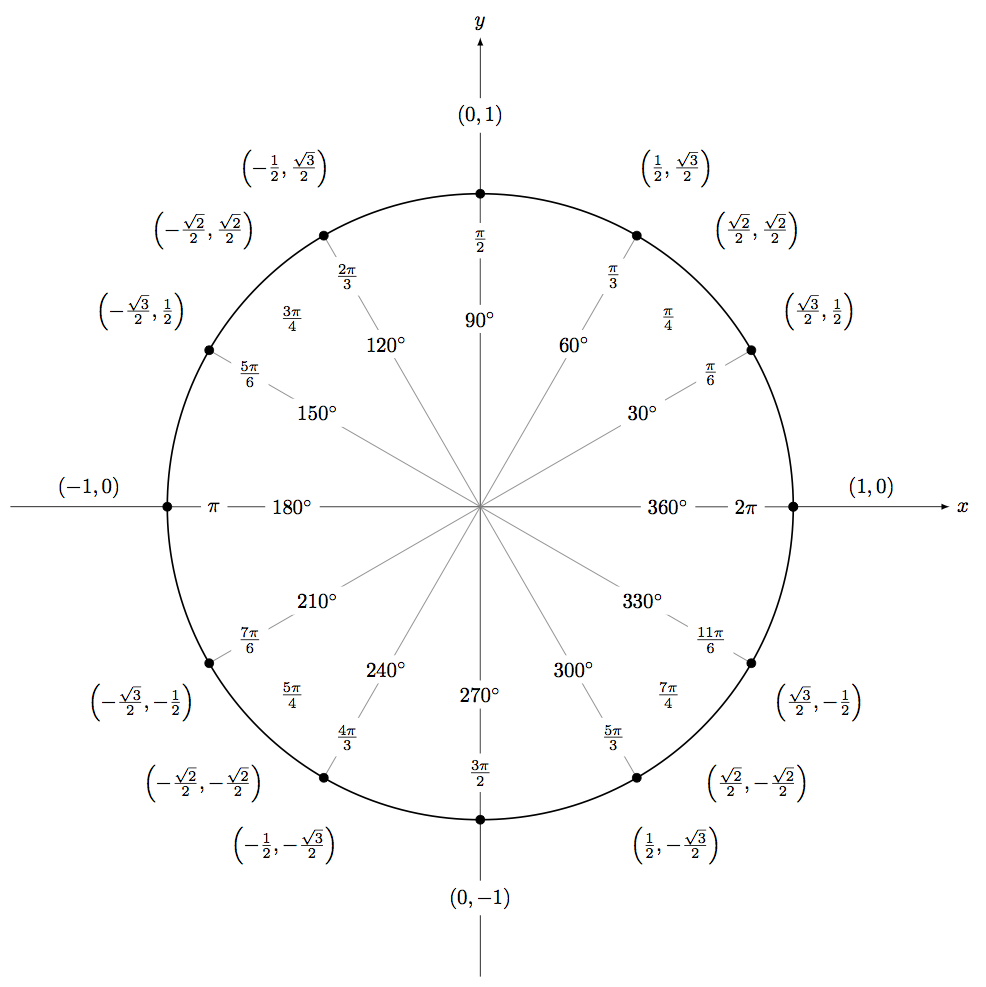
\includegraphics[scale=0.64]{unit_circle}
\newline\newline\newline\newline
\vfill
\columnbreak
\subsection {Other Information}
$ \frac{\sqrt{a}}{\sqrt{b}} = \sqrt{\frac{a}{b}} $\newline
Where a Cone is defined as $ z = \sqrt{a(x^2+y^2)}, $\newline
In Spherical Coordinates, $ \phi = \cos^{-1}(\sqrt{\frac{a}{1+a}}) $\newline
Right Circular Cylinder:\newline
$ V=\pi r^2h, SA=\pi r^2+2\pi rh $\newline
$ \lim_{n\to \inf} (1+\frac{m}{n})^{pn} = e^{mp} $\newline
Law of Cosines:\newline
$ a^2 = b^2 + c^2 - 2bc(\cos(\theta)) $

\subsection{Stokes Theorem}
Let:\newline
$\cdot$S be a 3D surface\newline
$\cdot\vec{F}(x,y,z) = M(x,y,z)\hat{i}+N(x,y,z)\hat{j}+P(x,y,z)\hat{l} $\newline
$\cdot$M,N,P have continuous $1^{st}$ order partial derivatives\newline
$\cdot$C is piece-wise smooth, simple, closed, curve, positively oriented\newline
$\cdot\hat{T}$ is unit tangent vector to C.\newline
Then,\newline
$ \oint\vec{F}_c\cdot\hat{T}dS = \int\int_s (\nabla\times\vec{F})\cdot\hat{n} dS = \int\int_R(\nabla\times\vec{F})\cdot\vec{n}dxdy $\newline
Remember:\newline
$ \oint\vec{F}\cdot\vec{T}ds = \int_c (Mdx + Ndy + Pdz) $

%The following can go away as needed, it is here so I can put my Accreditation message/source code message at the bottom right.
\vfill
{\fontsize{.5}{1}\selectfont Originally Written By Daniel Kenner for MATH 2210 at the University of Utah.\newline Source code available at https://github.com/keytotime/Calc3\_CheatSheet\newline Thanks to Kelly Macarthur for Teaching and Providing Notes.}
\end{multicols*}
\end{document}
